\documentclass[12pt,oneside]{report}

% =============================================================================
% PACKAGES
% =============================================================================
\usepackage[a4paper, margin=1in]{geometry}
\usepackage{graphicx}
\usepackage[hidelinks]{hyperref}
\usepackage{apacite}
\usepackage{booktabs}
\usepackage{array}
\usepackage[table]{xcolor}
\usepackage{fancyhdr}
\usepackage{lastpage}
\usepackage{float}
\usepackage{longtable}
\usepackage{url}
\usepackage{multirow}
\usepackage{makecell}
\usepackage{setspace}
\usepackage{titlesec}
\usepackage[toc,page]{appendix}
\usepackage{mathptmx}                 % Times New Roman font
\usepackage{tikz}                     % For architecture diagram
\usetikzlibrary{arrows.meta, positioning, shapes.geometric, calc}

% =============================================================================
% DOCUMENT SETTINGS
% =============================================================================

% Double spacing as required by template
\doublespacing

% Custom column types
\newcolumntype{C}[1]{>{\centering\arraybackslash}p{#1}}

% Colour-coded rating commands (for comparison tables)
\newcommand{\high}{\cellcolor{green!25}High}
\newcommand{\partialsupport}{\cellcolor{yellow!25}Partial}
\newcommand{\limited}{\cellcolor{orange!25}Limited}
\newcommand{\none}{\cellcolor{gray!25}None}

% Header and Footer
\setlength{\headheight}{14.5pt}
\pagestyle{fancy}
\fancyhf{}
\lhead{\textit{P2P Directory Synchronization}}
\rhead{\textit{Thesis}}
\cfoot{Page \thepage\ of \pageref{LastPage}}

% Chapter title style
\titleformat{\chapter}[display]
  {\normalfont\huge\bfseries}
  {\chaptertitlename\ \thechapter}{20pt}{\Huge}
\titlespacing*{\chapter}{0pt}{-20pt}{30pt}

% =============================================================================
% DOCUMENT
% =============================================================================
\begin{document}

% ---- Title Page ----
\begin{titlepage}
    \centering
    \vspace*{2cm}

    % Logo
    
\includegraphics[width=0.3\textwidth]{../screenshots/others/Epita.jpg}\\
    \vspace{1cm}

    % Title
    {\LARGE \textbf{Peer-to-Peer Directory Synchronization\\with Lightweight Version Control}}\\
    \vspace{1cm}

    % Team
    \large
    \begin{tabular}{c}
        Arihant Jain \\
        Su Huizhe \\
        Nizar Soufiya \\
        Shengkang Duan \\
    \end{tabular}

    \vspace{1.5cm}

    EPITA Graduate School of Computer Science\\
    \vspace{1cm}

    \textbf{Advisor}\\
    Thomas Broussard\\

    \vfill
    \today
\end{titlepage}

% ---- Declaration of Own Work ----
\newpage
\thispagestyle{empty}
\chapter*{Declaration of Own Work}
\addcontentsline{toc}{chapter}{Declaration of Own Work}

This work has been composed solely by us.

This work has not been accepted in any previous application for a degree or diploma, by Arihant Jain, Su Huizhe, Nizar Soufiya, and Shengkang Duan, or anyone else.

The work of which this is a record has been wholly done by us.

All extracts, including those created by generative AI, have been distinguished by quotation marks and the sources of our information have been specifically acknowledged and documented with in-text citations and in the bibliography.

All prompts with responses for any use Generative AI must be included in a separate MS Word document, clearly referencing its appearance in the bibliography and allowing the reader to easily associate the extract you used with the prompt. Here is how APA cites Generative AI: \url{https://apastyle.apa.org/blog/how-to-cite-chatgpt}

\vspace{0.8cm}

\begin{tabular}{p{6cm} p{6cm}}
Date: \underline{\hspace{4cm}} & \\[0.8cm]
Name: \underline{\hspace{4cm}} & Signature: \underline{\hspace{4cm}} \\[0.6cm]
Name: \underline{\hspace{4cm}} & Signature: \underline{\hspace{4cm}} \\[0.6cm]
Name: \underline{\hspace{4cm}} & Signature: \underline{\hspace{4cm}} \\[0.6cm]
Name: \underline{\hspace{4cm}} & Signature: \underline{\hspace{4cm}} \\[0.6cm]
\end{tabular}

% ---- Acknowledgements ----
\newpage
\chapter*{Acknowledgements}
\addcontentsline{toc}{chapter}{Acknowledgements}

We would like to thank our advisor for their guidance throughout this project. We also thank the EPITA faculty and Action Learning programme coordinators for providing the framework and resources that made this project possible. Finally, we thank each other for the late debugging sessions and the willingness to learn new languages and tools on a tight timeline.

% ---- Abstract / Executive Summary ----
\newpage
\chapter*{Abstract}
\addcontentsline{toc}{chapter}{Abstract}

Small collaborative teams, particularly university students working on temporary group projects, face a recurring problem: sharing and tracking project files without dedicated infrastructure. Cloud storage services require external servers and internet connectivity. Version control systems demand technical expertise and are designed for source code. Peer-to-peer file synchronization tools lack version history, meaning a single accidental overwrite can propagate to every connected device with no way to undo it.

This thesis proposes a peer-to-peer directory synchronization system with built-in version safety. The system discovers peers automatically on a local network using mDNS/DNS-SD, synchronizes file changes over direct TCP connections, and creates local backups before every synchronized overwrite. Conflict resolution uses a Last-Write-Wins policy paired with Lamport clock timestamps, a combination that keeps the implementation simple while ensuring no data is permanently lost.

The system is implemented as two cooperating daemons: a Go networking component handling peer discovery and synchronization coordination, and a C++ storage component handling file watching, content hashing, and disk I/O. A Java graphical frontend provides user visibility into synchronization status and version history.

% ---- Table of Contents ----
\newpage
\tableofcontents
\newpage

% ---- Chapters ----
\chapter{Introduction}

\section{Motivations}

The idea for this project came directly from discussions within our team. Arihant wanted to work on distributed systems, but the specific project proposal and application concept were developed by Su and Nizar based on real problems they observed. 

Specifically, Nizar observed this difficulty during EPITA's \emph{Challenge Week}. In a high-pressure team setting, group members who were unfamiliar with Git spent a lot of time troubleshooting setup issues, broken repositories, and merge conflicts. These technical hurdles regularly delayed collaboration, proving that for non-programmers or short-term work, Git is too complex to be practical.

At the same time, we saw the limits of simpler sharing methods. During a database course last semester, three of our team members ended up with four different versions of an ER diagram file. Reconciling those changes manually across email, WhatsApp, and USB drives was error-prone, and the final submission used an outdated version. 

Existing tools address parts of this problem. Google Drive \cite{googledrive} and Dropbox \cite{dropbox} synchronize files through cloud servers but require internet access, accounts, and have storage quotas. Git \cite{gitbook} tracks changes perfectly but requires advanced training in branches and staging. Syncthing \cite{syncthing} handles peer-to-peer transfers serverlessly, but it treats file version history as an afterthought and lacks a simple interface to undo accidental overwrites. 

Our goal was to build a tool that does all three: synchronize files automatically on a local network, protect files with automatic version backups before overwrites, and run with zero configuration or technical overhead.

\section{Context of the Project}

This project was developed as part of the Action Learning programme at EPITA, a programme that asks students to identify a real problem and build a solution in a team of four. Our team has two backend developers working in Go and C++, and two frontend and CI/CD developers working in Java with GitHub Actions.

The idea came from our own frustration. Rather than building something theoretical, we decided to solve the file-sharing problem we kept running into. The system we set out to build should feel invisible: put files into a folder on your laptop, and they show up on your teammates' laptops. Change a file, and everyone gets the update. If an update accidentally overwrites something, a backup of the old version is waiting in a local folder.

The Action Learning context shaped how we worked. With a fixed timeline and a small team, every design decision had to balance ambition against what could actually be built and tested in the available time.

\section{Objectives}

The project has three objectives:

\begin{enumerate}
    \item \textbf{Build a serverless synchronization system.} Peers discover each other automatically on a local network using mDNS/DNS-SD (the same protocols that let printers appear on your Wi-Fi without configuration). Files synchronize over direct TCP connections. No server, no accounts, no internet required.

    \item \textbf{Protect against accidental data loss.} Before any synchronized overwrite, the system saves the existing file into a local backup directory. Conflict resolution uses a Last-Write-Wins rule based on Lamport clock timestamps: predictable, automatic, and reversible.

    \item \textbf{Test two specific claims:}
    \begin{itemize}
        \item[$H_1$:] Average synchronization latency under one second on a standard WLAN for files up to 10\,MB, with no cloud infrastructure.
        \item[$H_2$:] For 3 to 5 peers, Lamport clocks with LWW are sufficient to maintain consistency and support rollback, without needing vector clocks or CRDTs.
    \end{itemize}
\end{enumerate}

\section{Overview of the Thesis}

Chapter~2 reviews the academic literature on distributed synchronization and collaborative file management. It discusses the trade-offs between different approaches and identifies the specific gap our project addresses.

Chapter~3 covers the state of the art: the research findings and technical decisions that determined our architecture, from protocol selection to conflict resolution strategy.

Chapter~4 describes the system architecture, how the Go and C++ components divide responsibilities, and how data flows through the system.

Chapter~5 explains the methodology, including our team structure, development process, tools, and the action plan for Action Learning Week.

Chapter~6 lists the expected development outcomes. After Action Learning Week, it will also cover what actually happened.

Chapter~7 presents the conclusions, summarises the contributions, and suggests directions for future work.

The appendices contain detailed comparison tables that support the analysis in Chapter~2.

\chapter{Literature Review}

This chapter covers the research that shaped our project. The goal is not to list tools or summarize papers, but to explain what the existing literature taught us and where it left questions that our project tries to answer.

The research was divided among the team. Arihant and Huizhe took on distributed systems theory: consistency models, replication strategies, and synchronization algorithms. They focused on the academic side, reading papers by Lamport, Shapiro, and Saito. Nizar and Shengkang surveyed existing tools and local networking technologies, testing products like Syncthing and comparing cloud platforms. Each week, we met to present what we found and argue about what mattered for our design. Some of the best design decisions came out of those arguments.

\section{The Collaborative File Management Landscape}

Collaborative file management tools can be grouped into four categories. None of them does everything well, and understanding where each one falls short is what pointed us toward our project.

\textbf{Centralized cloud platforms} (Google Drive \cite{googledrive}, Dropbox \cite{dropbox}, Nextcloud) are the tools most students reach for first. They synchronize files through a central server, handle multiple devices, and have friendly interfaces. The problems are structural, not cosmetic. Everything depends on the server. If the internet is down, or if the campus Wi-Fi drops, you cannot sync. If the provider changes their pricing or storage limits, you adjust or leave. Dropbox's own engineering team rebuilt their sync engine from scratch to handle the complexity of tracking file states across devices \cite{dropboxtech}, which illustrates how difficult reliable synchronization is even with centralised infrastructure. Version history exists, but it is time-limited (30 days on Google Drive, for example) and not designed for tracking the evolution of a project.

\textbf{Version control systems} (Git \cite{gitbook}, SVN, Perforce) solve the history problem completely. Git stores every version of every file, supports branching, and has detailed merge conflict resolution. But Git was built for software developers. The staging-committing-pushing workflow is not intuitive for someone who just wants to share a presentation or a dataset. In our own team, two out of four members had never used Git before this project, which is exactly the audience we are designing for.

\textbf{Peer-to-peer synchronization tools} (Syncthing \cite{syncthing}, Resilio Sync \cite{resilio}) take a different approach. They synchronize files directly between devices, no server needed. Syncthing in particular is open source, works on most platforms, and handles any file type. But when Nizar tested it for a week, he noticed a gap: if he accidentally saved a file with errors, it immediately replaced the file on all connected devices. Syncthing does have a versioning feature, but it is not on by default and the interface for recovering old versions is buried in the settings. Versioning is an afterthought, not part of the core design.

\textbf{Local sharing} (AirDrop, Nearby Share) is the simplest category. Select a file, tap a device, done. But these are one-shot transfers. There is no persistent connection, no synchronization, and no history. They solve a different problem.

The pattern is clear: each category does well on some dimensions and poorly on others. No single tool provides automatic synchronization, version safety, and zero configuration at the same time. The detailed comparison tables in Appendix~\ref{app:comparison-tables} show this across five evaluation dimensions.

\section{Synchronization in Distributed Systems}

Rather than providing a comprehensive survey of distributed systems literature, this section highlights the specific synchronization challenges and design trade-offs that guided our implementation.

\subsection{Ordering Events Without a Shared Clock}

The first problem any distributed system faces is ordering. When things happen on different machines, how do you decide what came first? Physical clocks are unreliable because machines drift.

Lamport \citeyear{lamport1978} proposed a simple solution: logical clocks. Each process keeps a counter and increments it on every event. When sending a message, the sender attaches its counter. The receiver updates its own counter to be at least as high. This creates a \emph{partial ordering}: if event $A$ causally led to event $B$, then $A$'s timestamp will always be lower.

The word ``partial'' matters. Lamport clocks cannot tell you whether two events are concurrent, that is, whether they happened independently with no causal connection. Fidge \citeyear{fidge1988} and Mattern independently proposed vector clocks to detect concurrency. Each node keeps an array of counters, one per participant. Vector clocks can identify concurrent events, but the counter array grows with the number of peers. Earlier, Parker et al. \citeyear{parker1983} had introduced version vectors for detecting mutual inconsistency between replicas, the formal basis for recognising when two copies of the same data have diverged.

For our system, this trade-off was the first real design decision. With 3 to 5 peers on a local network, vector clocks would mean carrying a small array of integers. The overhead is tiny. But vector clocks also require knowing all participants, and adding or removing a peer requires updating every node's vector. Since our system is designed for temporary groups where members join and leave, Lamport clocks are simpler to manage. The cost is that we cannot detect true concurrency. If two peers edit the same file at the exact same moment, one version will silently overwrite the other. The backup mechanism makes this acceptable, but it is a real limitation.

\subsection{The CAP Theorem and Why It Matters}

Gilbert and Lynch \citeyear{brewer2002} proved that a distributed system cannot simultaneously guarantee consistency, availability, and partition tolerance. During a network partition (which on a campus Wi-Fi happens every time a laptop lid closes), you must choose: either block operations until the partition heals (consistency), or allow operations to continue and reconcile later (availability).

In our case, we have to prioritize availability. Student laptops disconnect constantly: Wi-Fi drops, people move between classrooms, or a battery dies. If the sync tool blocked edits whenever a teammate was offline, it would be unusable. We therefore accept eventual consistency, allowing each peer to edit files offline and sync changes once they reconnect.

Vogels \citeyear{vogels2009} argued that eventual consistency is the right model for applications where reading slightly stale data is harmless. A teammate seeing a file that is ten seconds out of date causes no damage. Losing a file because the system refused to save it during a disconnection does.

\subsection{Resolving Conflicts}

When two peers edit the same file while disconnected, the system must decide what happens when they reconnect. The literature offers several approaches, each with trade-offs.

\textbf{Operational transformation} (OT) \cite{sun1998} tracks individual editing operations (insert character at position 5, delete characters 3 through 7) and transforms them so they can be applied in any order. Google Docs relies on this. OT is powerful for text, but it requires operation-level logging. For binary files like images, spreadsheets, or compiled code, there are no ``operations'' to transform.

\textbf{CRDTs} (Conflict-free Replicated Data Types) \cite{shapiro2011} are data structures that mathematically guarantee convergence. Shapiro et al. proved that any data type whose merge operation is commutative, associative, and idempotent will converge regardless of operation order. This is a strong result. But applying CRDTs to file metadata requires defining what ``merge'' means for each field in the metadata schema, and testing the merge logic thoroughly.

\textbf{Last-Write-Wins} (LWW) is the simplest policy: keep the version with the highest timestamp. One version is discarded. The Bayou project \cite{bayou1995} demonstrated that LWW becomes safe when combined with backup storage: before overwriting a file, save the old copy somewhere. Terry et al. \citeyear{terry1994} added ``session guarantees,'' ensuring that a user always sees the results of their own writes, even if other peers' updates have not arrived.

After reading these papers, the team debated for two meetings before settling on LWW with backups. CRDTs would be technically better, but implementing and testing them correctly within our timeline was unrealistic. Saito and Shapiro's \citeyear{saito2005} survey of optimistic replication confirmed that our approach, optimistic local updates with deferred reconciliation and rollback, is a well-documented pattern for weakly connected systems. That reassured us. The metadata schema we designed can support CRDTs in a future version, using register-based merge semantics from Shapiro et al. \citeyear{shapiro2011}, so the option remains open.

\subsection{Propagating Updates Efficiently}

Tridgell and Mackerras \citeyear{rsync1996} showed that rolling checksums allow two machines to identify which \emph{blocks} of a file have changed and transfer only the differences. This is the core idea behind rsync, and it reduces bandwidth use dramatically for large files with small changes.

Demers et al. \citeyear{demers1987} studied a separate problem: how to reliably spread updates across a group of peers without a central coordinator. Their ``epidemic'' (gossip) algorithms model updates as a contagion that spreads from peer to peer until everyone has it. The approach is probabilistic but robust, and it scales well.

For our initial version, we transfer whole files. It is simpler to implement, simpler to debug, and for files under a few megabytes on a local network, the performance penalty is small. The architecture is designed to support both optimizations later: block-level transfers in the C++ daemon, and gossip propagation in the Go coordinator.

\section{Identified Gap}

Comparing existing tools across five dimensions (membership management, synchronization capability, history management, file type support, and filesystem transparency) shows a consistent pattern. The full tables are in Appendix~\ref{app:comparison-tables}; here is the summary:

\begin{itemize}
    \item Cloud platforms score well on synchronization and usability, but poorly on history management and offline use.
    \item Version control systems score well on history, but poorly on synchronization automation and accessibility for non-technical users.
    \item P2P sync tools score well on synchronization and usability, but poorly on history management.
    \item Local sharing tools score well on usability but offer no synchronization or history at all.
\end{itemize}

The gap is not that any single feature is missing from the market. It is that no tool scores well across all five dimensions simultaneously. Each existing tool was optimised for a different audience (enterprise workers, developers, power users, casual sharers), leaving a gap for small, temporary teams who want something that ``just works'' on a local network with version safety included.

\section{Positioning the Project}

Our system targets this gap. It differs from existing tools in four concrete ways:

\begin{itemize}
    \item \textbf{LAN-only, serverless operation.} Peer discovery uses mDNS/DNS-SD on the local subnet. No servers, accounts, or internet connection needed.
    \item \textbf{Zero configuration.} Peers appear automatically. There is nothing to install per-project, no folder IDs to share, no repositories to initialise.
    \item \textbf{Automatic version backups.} Every overwrite saves the old file first. This is built into the synchronization protocol, not a feature that must be turned on.
    \item \textbf{Low-resource split architecture.} Go handles networking (peer coordination, TCP connections). C++ handles file I/O (watching, hashing, disk writes). This keeps CPU and memory use low on student laptops.
\end{itemize}

Three design principles guide the project:

\begin{enumerate}
    \item \textbf{Transparency.} The synchronized folder should look and feel like a normal local folder. No special commands. No merge dialogs.
    \item \textbf{Safety.} If the system changes a file, the old version must be recoverable. No automation should cause permanent data loss.
    \item \textbf{Lightness.} The tool runs continuously in the background. It must not drain battery life or make the laptop feel slow.
\end{enumerate}

\section{Summary}

The literature review taught us three things that directly determined the design of this project.

The CAP theorem says we must accept eventual consistency. Students disconnect constantly, and a synchronization tool that stops working when someone closes their laptop is useless. The system has to let everyone work offline and sort out differences later.

For conflict resolution, the right choice depends on scale and timeline. LWW with backups gives us simple, predictable behaviour with no risk of permanent data loss. CRDTs would be better for a production system, but they are complex to implement correctly. The schema supports adding them later.

No existing tool occupies the design space we are targeting. Cloud services, version control, P2P sync, and local sharing each solve part of the problem. None of them solve all of it at once, for a small team, on a local network, with no setup. That is where our project fits.

\chapter{State of the Art and Design Choices}

\section{Summary}
\label{sec:state-of-art-summary}

This chapter documents the state of the art that emerged from our research. It covers the technology choices, architecture decisions, and synchronization strategies adopted for this project, with citations and critical assessment for each. Where Chapter~2 surveyed the landscape and identified the gap, this chapter explains how the research translated into concrete design decisions. Table~\ref{tab:research-mapping} shows how each research finding maps to a component in the system.

\begin{table}[htbp]
\centering
\caption{Research-to-Implementation Mapping}
\label{tab:research-mapping}
\begin{tabular}{p{4.5cm} p{4cm} p{5cm}}
\toprule
\textbf{Research Finding} & \textbf{Source} & \textbf{System Component} \\
\midrule
Zero-config discovery & RFC 6762/6763 & Go mDNS broadcaster \\
\midrule
Causal event ordering & Lamport (1978) & Per-file Lamport counters \\
\midrule
Partition tolerance & CAP theorem (2002) & Offline-first availability \\
\midrule
Conflict resolution & Bayou (1995) & LWW + local backups \\
\midrule
Optimistic replication & Saito \& Shapiro (2005) & State-transfer architecture \\
\midrule
Delta sync (future) & rsync (1996) & Planned block-level sync \\
\midrule
File change detection & inotify / FSEvents & C++ kernel watchers \\
\midrule
Data integrity & SHA-256 / TCP & C++ hashing + Go TCP pools \\
\bottomrule
\end{tabular}
\end{table}

\section{Zero-Configuration Peer Discovery}

Multicast DNS (mDNS) and DNS-Based Service Discovery (DNS-SD) \cite{rfc6762, rfc6763} are the protocols that allow devices on a local network to find each other without a central server. They are the reason a printer shows up on your laptop's Wi-Fi list without anyone typing in its IP address.

Our Go discovery component broadcasts a service record under the \texttt{\_p2psync.\_tcp} domain and continuously browses the subnet for other instances. When a new peer appears, its address is resolved automatically. Users never see an IP address, a device ID, or an invitation code.

Why mDNS and not something else? During the research phase, Nizar looked into how Syncthing handles discovery. Syncthing uses a combination of local discovery and global relay servers. The local part is effective, but the global relay adds complexity and an external dependency. Since our target environment is a campus Wi-Fi where all team members are on the same subnet, mDNS gives us what we need without any external infrastructure \cite{syncthing}.

There is a known limitation. Some enterprise Wi-Fi networks block multicast traffic. On EPITA's campus network, multicast works without issues. For networks that block it, a fallback would be needed, but adding a relay server would contradict the serverless design goal. For now, we accept this limitation and document it.

\section{Event Ordering with Lamport Clocks}

Every file in the system carries a Lamport counter in its metadata \cite{lamport1978}. When a peer modifies a file, it increments the counter and includes the new value in the synchronization message. A receiving peer compares the incoming counter against its local value. If the incoming number is higher, the file is newer.

This is the same mechanism described in Section~2.2.1, applied at the per-file level. The counter is stored in the local SQLite metadata database alongside the file's SHA-256 hash and path.

One design question came up during implementation: should the counter be global (one counter per peer, shared across all files) or per-file? A global counter would increment even when unrelated files change, leading to unnecessary updates. A per-file counter only increments when that specific file changes, which keeps the update traffic proportional to actual changes. After discussing it in a team meeting, the per-file approach won.

The limitation is unchanged: Lamport clocks cannot detect concurrent edits. If Arihant edits \texttt{report.pdf} on his laptop while Huizhe edits the same file on his, and neither has seen the other's change, the timestamps do not tell the system that a conflict exists. The LWW tiebreaker picks one version, and the backup mechanism saves the other. Fidge's \citeyear{fidge1988} vector clocks would detect the concurrency, but at the cost of carrying an array of counters that must be updated whenever the peer group changes.

\section{Availability Over Consistency}

The CAP theorem \cite{brewer2002} forced a clear decision: prioritise availability. Peers must be able to edit files freely whether or not other peers are reachable. Reconciliation happens when connectivity returns.

In practice, this means the system is ``eventually consistent'' in the sense described by Vogels \citeyear{vogels2009}. A peer that goes offline for an hour can accumulate many local changes. When it reconnects, the Go daemon exchanges metadata with other peers and pulls in any files that have newer timestamps. If a conflict exists, LWW resolves it automatically and the backup directory preserves the losing version.

The risk of eventual consistency is that two peers may briefly see different versions of the same file. For our use case, this is acceptable. A project team member seeing a file from ten seconds ago is fine. A system that prevents editing during a Wi-Fi dropout is not.

\section{Last-Write-Wins with Version Backups}

Conflict resolution uses LWW, following the approach from Bayou \cite{bayou1995}. Before the C++ daemon writes an incoming file to disk, it copies the existing local version into a \texttt{.versions/} subdirectory, tagged with a timestamp. This ensures that LWW never causes permanent data loss.

Saito and Shapiro \citeyear{saito2005} classify our approach as ``state transfer with rollback support.'' State transfer means sending entire file states (as opposed to operation transfer, which sends edit deltas). It is simpler to implement and debug, though it uses more bandwidth.

The team considered three alternatives before settling on LWW:

\begin{enumerate}
    \item \textbf{Manual conflict resolution} (like Git): rejected because it requires user intervention, which defeats the goal of invisible synchronization.
    \item \textbf{CRDTs} \cite{shapiro2011}: rejected for the initial version due to implementation complexity, but the metadata schema is designed to support register-based CRDTs in a future iteration.
    \item \textbf{Rename-on-conflict} (like Dropbox's ``conflicted copy''): considered, but it creates confusing duplicate files. LWW with backups achieves the same safety without cluttering the working directory.
\end{enumerate}

\section{File Change Detection}

Polling a directory for changes is wasteful. It consumes CPU cycles even when nothing has changed, and the polling interval adds latency. Modern operating systems provide kernel-level event APIs: inotify on Linux \cite{inotify7} and FSEvents on macOS \cite{fsevents}.

The C++ daemon registers watchers on the synchronization directory and all its subdirectories. When a file is created, modified, or deleted, the kernel pushes an event. The daemon debounces rapid sequences of events (common when saving a file triggers multiple write operations) and forwards a consolidated update to the Go daemon through IPC.

This gives near-instant detection. In informal tests on Arihant's MacBook, the delay between saving a file and the Go daemon receiving the metadata update was consistently under 50 milliseconds.

\section{Data Integrity and Network Transport}

Every file has a SHA-256 hash \cite{fips1804} computed by the C++ daemon using memory-mapped I/O. The hash serves two purposes: detecting changes (if the hash is different, the file has changed) and verifying integrity after transfer (the receiver recomputes the hash and compares).

Network transport uses TCP \cite{rfc9293}. The Go daemon maintains a pool of TCP connections with discovered peers. When a file transfer is needed, the Go daemon establishes the connection and hands the socket to the C++ daemon, which streams the file data directly to disk. TCP's built-in flow control and error recovery mean we do not need to implement our own retransmission logic.

Whole-file transfer is the initial design. The rsync algorithm \cite{rsync1996} could reduce bandwidth by transferring only changed blocks, but implementing it correctly adds significant complexity. The architecture has a clean separation between the networking layer (Go) and the storage layer (C++), so adding block-level transfers later would only require changes in the C++ daemon.


\chapter{System Architecture}

\section*{Summary}
This chapter describes the design adopted to achieve the objectives stated in the Introduction. The architecture splits the system into two cooperating processes, a Go networking daemon and a C++ storage daemon, connected by inter-process communication. A Java frontend provides the user interface. Figure~\ref{fig:architecture} shows how the components relate to each other.

\section{System Architecture Anticipated}
\label{sec:arch-anticipated}

\subsection{Component Overview}

The decision to use two separate daemons was not arbitrary. Go has strong support for networking, concurrency, and cross-platform compilation, making it well-suited for peer discovery and synchronization coordination. C++ provides the low-level control needed for memory-mapped file I/O, kernel event APIs, and high-performance hashing. Running them as separate processes also means a crash in one does not take down the other.

\begin{enumerate}
    \item \textbf{Go Networking Daemon.} Responsible for mDNS/DNS-SD peer discovery, managing TCP connection pools with discovered peers, coordinating which files need to be synchronised, and running the IPC server that the C++ daemon and Java frontend connect to.

    \item \textbf{C++ Storage Daemon.} Responsible for kernel-level file watching (inotify on Linux, FSEvents on macOS), computing SHA-256 hashes with memory-mapped I/O, creating version backups before overwrites, and streaming incoming files directly to disk from TCP sockets.

    \item \textbf{Java Frontend.} A desktop application showing the current synchronization status, the list of connected peers, a file-by-file version history, and controls for choosing the synchronization directory. It communicates with the Go daemon through IPC.
\end{enumerate}

\subsection{Architecture Diagram}

\begin{figure}[htbp]
\centering
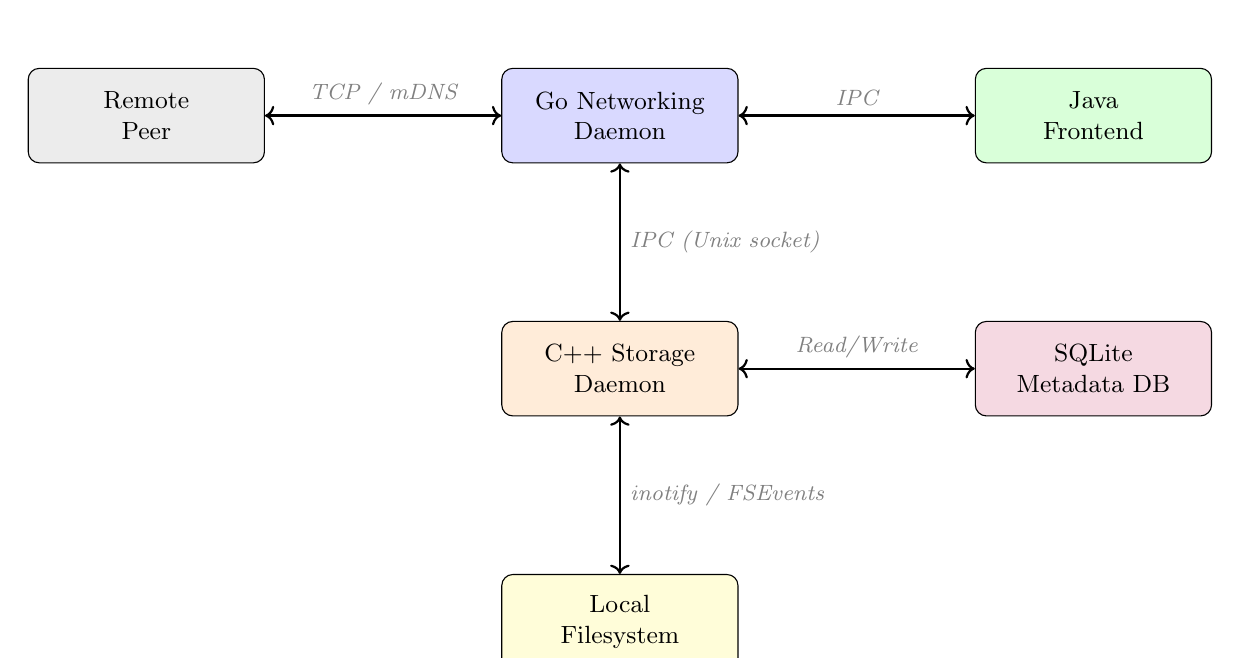
\begin{tikzpicture}[
    node distance=1.5cm and 2.5cm,
    component/.style={draw, rounded corners, minimum width=3cm, minimum height=1.2cm, align=center, font=\small},
    label/.style={font=\footnotesize\itshape, text=gray},
    arrow/.style={-{Stealth[length=3mm]}, thick}
]

% Go Daemon
\node[component, fill=blue!15] (go) {Go Networking\\Daemon};

% C++ Daemon
\node[component, fill=orange!15, below=2cm of go] (cpp) {C++ Storage\\Daemon};

% Java Frontend
\node[component, fill=green!15, right=3cm of go] (java) {Java\\Frontend};

% Remote Peer
\node[component, fill=gray!15, left=3cm of go] (peer) {Remote\\Peer};

% Filesystem
\node[component, fill=yellow!15, below=2cm of cpp] (fs) {Local\\Filesystem};

% SQLite
\node[component, fill=purple!15, right=3cm of cpp] (db) {SQLite\\Metadata DB};

% Connections
\draw[arrow, <->] (go) -- node[right, label] {IPC (Unix socket)} (cpp);
\draw[arrow, <->] (go) -- node[above, label] {IPC} (java);
\draw[arrow, <->] (go) -- node[above, label] {TCP / mDNS} (peer);
\draw[arrow, <->] (cpp) -- node[right, label] {inotify / FSEvents} (fs);
\draw[arrow, <->] (cpp) -- node[above, label] {Read/Write} (db);

\end{tikzpicture}
\caption{System architecture showing the Go networking daemon, C++ storage daemon, Java frontend, and their communication channels.}
\label{fig:architecture}
\end{figure}

\subsection{Synchronization Data Flow}

A typical synchronization cycle proceeds through eight steps:

\begin{enumerate}
    \item The C++ daemon detects a file change through a kernel event and computes the new SHA-256 hash.
    \item It sends a metadata update (file path, new hash, incremented Lamport timestamp) to the Go daemon through IPC.
    \item The Go daemon broadcasts the metadata to all connected peers over TCP.
    \item Each receiving peer compares the incoming timestamp against its local copy.
    \item If the incoming version is newer, the receiving Go daemon requests the full file from the sender.
    \item The file data is streamed over TCP directly to the receiving C++ daemon.
    \item Before writing the incoming file to disk, the receiving C++ daemon copies the existing version to the \texttt{.versions/} directory.
    \item The new file is written, and the local SQLite metadata database is updated.
\end{enumerate}

\subsection{Metadata Storage}

Each peer maintains a local SQLite database. The schema stores one row per tracked file:

\begin{itemize}
    \item \textbf{path}: file path relative to the sync root
    \item \textbf{sha256}: content hash (32 bytes, hex-encoded)
    \item \textbf{lamport\_ts}: the file's Lamport clock value (integer)
    \item \textbf{mtime}: last modification time (for display; not used for ordering)
    \item \textbf{size}: file size in bytes
\end{itemize}

The schema was designed with future extensibility in mind. Adding columns for CRDT state (e.g., a vector of per-peer counters) would not require restructuring the synchronization protocol.

\subsection{Communication Protocols}

Four communication channels are used:

\begin{itemize}
    \item \textbf{Discovery:} mDNS multicast on port 5353, advertising the \texttt{\_p2psync.\_tcp} service type.
    \item \textbf{Coordination:} A lightweight custom protocol over TCP for exchanging file metadata (file lists, version comparisons, transfer requests).
    \item \textbf{File Transfer:} Direct TCP streaming. The Go daemon sets up the connection; the C++ daemon handles the actual file I/O.
    \item \textbf{Internal IPC:} Unix domain sockets between the Go and C++ daemons on the same machine.
\end{itemize}

\section{System Architecture Updated}
\label{sec:arch-updated}

\textit{This section will be completed at the end of Action Learning Week. It will document changes to the architecture that emerged during implementation: what worked as planned, what had to be modified, and what lessons came from the integration process.}

\chapter{Methodology}

\section*{Summary}
This chapter describes the methodology used in the project, the stages by which it was implemented, and the research design. It details the participants, the tools and instruments used, the development procedure, and how results will be evaluated. The action plan for Action Learning Week is included at the end.

\section{Methodology Anticipated}
\label{sec:method-anticipated}

\subsection{Team Structure and Roles}

The team has four members. Responsibilities were divided by technical domain, based on each member's existing skills and what they wanted to learn:

\begin{itemize}
    \item \textbf{Arihant Jain} (Backend, Go): peer discovery, synchronization coordination, IPC server, TCP networking. Arihant had prior experience with Go from a personal project and took the lead on the networking daemon.
    \item \textbf{Su Huizhe} (Backend, C++): file watching, SHA-256 hashing, file versioning, disk I/O. Huizhe had worked with C++ in systems programming courses and was comfortable with memory-mapped I/O and kernel APIs.
    \item \textbf{Nizar Soufiya} (Frontend, Java): user interface design and implementation. Nizar had experience with Java Swing from a previous course project.
    \item \textbf{Shengkang Duan} (Frontend and CI/CD, Java): build automation, test pipeline, GitHub Actions configuration. Shengkang set up the continuous integration pipeline early in the project, which gave the team fast feedback on every commit.
\end{itemize}

The split between backend and frontend roughly corresponds to the Go/C++ daemons and the Java GUI described in Chapter~4. The two groups worked in parallel for most of the project, meeting weekly to align on interface contracts and integration issues.

\subsection{Development Process}

Rather than writing a detailed specification and implementing it sequentially, the team followed an iterative development process structured around the course milestones from April to July 2026. The project moved through four distinct phases:

\begin{enumerate}
    \item \textbf{Phase 1: Initiation and Research (April 19 to May 15, 2026).} Began with the Project Proposal submission on April 19, followed by the Literature Review and Presentation Workshop on April 28. During this phase, we divided research areas, submitted our initial bibliography on May 8, and outlined the literature review on May 15. The focus was on studying distributed systems algorithms (such as logical clocks and CAP theorem trade-offs) and testing local network discovery protocols (mDNS/DNS-SD).
    
    \item \textbf{Phase 2: Core Prototyping (May 6 to May 29, 2026).} Initiated at Hackathon 1 (Prototype Sprint) on May 6, where we wrote the first standalone prototypes of the Go networking module and the C++ file-watching daemon. The theoretical foundation was finalized and submitted as the Completed Literature Review on May 29.
    
    \item \textbf{Phase 3: Integration and MVP Sprints (June 12 to June 22, 2026).} Following the Public Speaking Workshop on June 12, we completed Hackathon 2 (MVP Sprint) on June 17, which focused on end-to-end integration over Unix domain sockets. This phase culminated in the submission of this thesis and the accompanying Gen AI documentation on June 22.
    
    \item \textbf{Phase 4: Live Evaluation (July 6 to July 10, 2026).} Scheduled for Action Learning Week, this final phase consists of live WLAN latency and consistency testing, concluding on July 10 with the submission of the final MVP, 360 peer evaluations, and poster presentation.
\end{enumerate}

\begin{table}[htbp]
\centering
\caption{Action Learning Project Milestones}
\label{tab:milestones}
\begin{tabular}{p{4.5cm} p{8.5cm}}
\toprule
\textbf{Milestone / Event} & \textbf{Date / Deadline} \\
\midrule
Project Proposal Submission & April 19, 2026 \\
\midrule
Literature Review Workshop & April 28, 2026 (In-person) \\
\midrule
Hackathon 1 (Prototype Sprint) & May 6, 2026 (In-person) \\
\midrule
Bibliography Submission & May 8, 2026 \\
\midrule
Literature Review Outline & May 15, 2026 \\
\midrule
Completed Literature Review & May 29, 2026 \\
\midrule
Public Speaking Workshop & June 12, 2026 \\
\midrule
Hackathon 2 (MVP Sprint) & June 17, 2026 (In-person) \\
\midrule
Thesis \& Gen AI Submission & June 22, 2026 \\
\midrule
Action Learning Week & July 6 to 10, 2026 (In-person) \\
\midrule
Final MVP, Poster \& 360 Eval & July 10, 2026 \\
\bottomrule
\end{tabular}
\end{table}

\subsection{Tools and Instruments}

\begin{table}[htbp]
\centering
\caption{Development Tools}
\label{tab:tools}
\begin{tabular}{p{4cm} p{9cm}}
\toprule
\textbf{Category} & \textbf{Tool} \\
\midrule
Languages & Go 1.21+, C++17, Java 17 \\
\midrule
Build systems & Go modules, CMake (C++), Gradle (Java) \\
\midrule
Version control & Git with GitHub for hosting and code review \\
\midrule
CI/CD & GitHub Actions (build, lint, test on every push) \\
\midrule
Testing frameworks & Go \texttt{testing} package, Google Test (C++), JUnit 5 (Java) \\
\midrule
Test environment & 3 to 5 laptops on the same WLAN subnet \\
\midrule
Documentation & \LaTeX\ (thesis and literature review) \\
\bottomrule
\end{tabular}
\end{table}

\subsection{Research Design}

The project tests two hypotheses through controlled experiments:

\textbf{Hypothesis 1 (Latency):} Measure the time from a file being saved on one peer to it appearing on another, across 3 to 5 peers connected to the same WLAN. Success is defined as sub-second average latency for files up to 10\,MB. The test procedure involves saving files of different sizes (1\,KB, 100\,KB, 1\,MB, 10\,MB) and recording timestamps at both ends.

\textbf{Hypothesis 2 (Consistency):} Simulate concurrent edits by having two peers modify the same file while disconnected, then reconnecting them. Success is defined by three criteria: (a) no file is permanently lost due to conflict resolution, (b) all peers converge to the same version within 30 seconds of reconnection, and (c) the overwritten version is recoverable from the \texttt{.versions/} backup directory.

\subsection{Action Plan}

Table~\ref{tab:action-plan} maps the work to the Action Learning Week timeline.

\begin{table}[htbp]
\centering
\caption{Action Plan for Action Learning Week}
\label{tab:action-plan}
\begin{tabular}{p{3cm} p{10cm}}
\toprule
\textbf{Period} & \textbf{Planned Work} \\
\midrule
Pre-ALW & Literature review complete, architecture finalised, Go and C++ prototypes built and tested independently \\
\midrule
ALW Days 1 and 2 & IPC integration between Go and C++ daemons; first end-to-end sync test between two laptops \\
\midrule
ALW Days 3 and 4 & Multi-peer testing (3+ laptops); Java frontend integration; conflict simulation tests \\
\midrule
ALW Day 5 & Hypothesis evaluation (latency testing, consistency validation); documentation of results \\
\bottomrule
\end{tabular}
\end{table}

\section{Methodology Updated}
\label{sec:method-updated}

\textit{This section will be completed at the end of Action Learning Week. It will describe what actually happened: which parts of the plan worked, what had to change, what problems came up, and how the team adapted.}

\chapter{Results}

\section*{Summary}
This chapter details the results of what was learned and accomplished during the project.

\section{Development Anticipated}
\label{sec:results-anticipated}

Based on the architecture in Chapter~4 and the methodology in Chapter~5, the following development outcomes are planned:

\textbf{Go Networking Daemon.} A working daemon that discovers peers on the local subnet through mDNS/DNS-SD, maintains persistent TCP connections with them, exchanges file metadata to detect changes, coordinates file transfers, and communicates with the C++ daemon through Unix domain sockets. The core packages (\texttt{discovery}, \texttt{network}, \texttt{ipc}) are already prototyped and tested independently; integration is the remaining work.

\textbf{C++ Storage Daemon.} A working daemon that watches the synchronization directory using kernel-level APIs (inotify on Linux, FSEvents on macOS), computes SHA-256 hashes of modified files with memory-mapped I/O, saves existing files to a \texttt{.versions/} directory before any overwrite, and streams incoming file data directly from TCP sockets to disk.

\textbf{Java Frontend.} A desktop application that shows the current synchronization status (which peers are connected, which files are syncing), displays a per-file version history with the ability to restore a previous version, and lets users configure the synchronization directory.

\textbf{Hypothesis Testing.} Two sets of measurements:
\begin{itemize}
    \item $H_1$ (Latency): timed synchronization tests across 3 to 5 peers on the campus WLAN, for files ranging from 1\,KB to 10\,MB. Target: sub-second average latency.
    \item $H_2$ (Consistency): concurrent edit scenarios where two peers modify the same file while disconnected, then reconnect. Expected outcome: automatic resolution with no permanent data loss, convergence within 30 seconds, and full recoverability from backups.
\end{itemize}

\section{Development Updated}
\label{sec:results-updated}

\textit{This section will be completed at the end of Action Learning Week in a separate standalone document. It will describe the differences between what was anticipated above and what was actually developed: features that were completed, features that were modified, and features that were deferred. Maximum one-half page.}

\chapter{Conclusions}

When this project started, the problem seemed straightforward: build a tool that lets a small group of students share files on a local network without setting up servers or learning Git. The research and design process revealed that the problem is more nuanced than it appears. Distributed synchronization, even for a handful of peers, touches on event ordering, consistency models, and conflict resolution, all topics with decades of research behind them.

The literature review (Chapter~2) showed that existing tools each solve part of the problem. Cloud services handle synchronization well but depend on external infrastructure. Git handles versioning well but requires technical expertise. Syncthing handles peer-to-peer transfer well but treats versioning as an afterthought. No existing tool scores well across all five evaluation dimensions (membership, synchronization, history, file support, and transparency) simultaneously.

The system described in this thesis fills that gap. The Go networking daemon discovers peers through mDNS/DNS-SD and coordinates synchronization using per-file Lamport clocks with Last-Write-Wins conflict resolution. The C++ storage daemon watches the filesystem for changes, computes content hashes, and creates backups before every overwrite. The Java frontend shows users what is happening without requiring them to understand the underlying protocols.

The design makes three deliberate trade-offs:

\begin{itemize}
    \item \textbf{Lamport clocks instead of vector clocks.} Simpler to implement and manage when peers join and leave, but unable to detect truly concurrent edits.
    \item \textbf{LWW instead of CRDTs.} One version is chosen automatically; the other is preserved in a backup. Simple and predictable, but not conflict-free in the CRDT sense.
    \item \textbf{Whole-file transfers instead of delta sync.} Easy to implement and debug, but wasteful for large files with small changes.
\end{itemize}

Each of these trade-offs is appropriate for 3 to 5 peers on a local network with a project timeline of a few months. A production system serving hundreds of users would need to revisit all three.

Several directions for future work remain:

\begin{itemize}
    \item \textbf{Block-level delta synchronization.} Implementing the rsync rolling-checksum algorithm in the C++ daemon to transfer only changed blocks, reducing bandwidth for large files.
    \item \textbf{CRDT-based metadata.} Extending the SQLite schema to use state-based CRDTs for file metadata, enabling conflict-free convergence without LWW.
    \item \textbf{Cross-subnet discovery.} Supporting peers on different subnets, possibly through a lightweight relay, while preserving zero-configuration on local networks.
    \item \textbf{Mobile support.} Adapting the architecture for Android and iOS, where background execution and filesystem access are more restricted than on desktop operating systems.
\end{itemize}

What this project demonstrates is that the individual building blocks for lightweight peer-to-peer synchronization, mDNS, Lamport clocks, LWW, TCP, SHA-256, are well-understood and well-documented. The challenge is not inventing new algorithms. It is combining existing ones into a package that is simple enough for non-technical users, safe enough that no data is lost, and light enough to run unnoticed on a student laptop. That is what this system sets out to do.


% ---- Bibliography ----
\newpage
\bibliographystyle{apacite}
\bibliography{thesis}

% ---- Appendices ----
\begin{appendices}

\chapter{Detailed Comparison Tables}
\label{app:comparison-tables}

The following tables provide a detailed, dimension-by-dimension comparison of existing collaborative file management approaches. They supplement the analysis presented in Chapter~2 by providing granular ratings for individual systems within each category.

The qualitative ratings used are defined in Table~\ref{tab:rating-scale-app}.

\begin{table}[htbp]
\centering
\caption{Qualitative Rating Scale}
\label{tab:rating-scale-app}
\begin{tabular}{cc}
\toprule
\textbf{Rating} & \textbf{Meaning} \\
\midrule
\high & Strong support for the capability \\
\partialsupport & Partial support with notable limitations \\
\limited & Basic or restricted support \\
\none & Capability not provided \\
\bottomrule
\end{tabular}
\end{table}

% ---------- Membership Management ----------
\begin{table}[htbp]
\centering
\caption{Comparison: Membership Management}
\label{tab:app-membership}
\begin{tabular}{
C{2.3cm}
C{2.3cm}
C{3.2cm}
C{3.2cm}
C{3.2cm}
}
\toprule
\textbf{Category} & \textbf{System} & \makecell{\textbf{Peer}\\\textbf{Discovery}} & \makecell{\textbf{Access}\\\textbf{Control}} & \makecell{\textbf{Group}\\\textbf{Formation}} \\
\midrule
\multirow{4}{*}{Centralized}
& \textit{Google Drive}  & \limited & \high & \high \\
& \textit{OneDrive}      & \limited & \high & \high \\
& \textit{Dropbox}       & \limited & \high & \high \\
& \textit{Nextcloud}     & \limited & \high & \partialsupport \\
\midrule
\multirow{3}{*}{Version Control}
& \textit{Git}       & \none & \none & \limited \\
& \textit{SVN}       & \none & \high & \limited \\
& \textit{Perforce}  & \none & \high & \limited \\
\midrule
\multirow{2}{*}{P2P Sync}
& \textit{Syncthing}     & \high & \partialsupport & \partialsupport \\
& \textit{Resilio Sync}  & \partialsupport & \partialsupport & \partialsupport \\
\midrule
\multirow{2}{*}{Local Sharing}
& \textit{AirDrop}       & \high & \none & \limited \\
& \textit{Nearby Share}  & \high & \none & \limited \\
\bottomrule
\end{tabular}
\end{table}

% ---------- Synchronization Model ----------
\begin{table}[htbp]
\centering
\caption{Comparison: Synchronization Model}
\label{tab:app-sync}
\begin{tabular}{
C{2.3cm}
C{2.3cm}
C{3.2cm}
C{3.2cm}
C{3.2cm}
}
\toprule
\textbf{Category} & \textbf{System} & \makecell{\textbf{Automatic}\\\textbf{Sync}} & \makecell{\textbf{Offline}\\\textbf{Operation}} & \makecell{\textbf{Multi-Device}\\\textbf{Sync}} \\
\midrule
\multirow{4}{*}{Centralized}
& \textit{Google Drive}  & \high & \limited & \high \\
& \textit{OneDrive}      & \high & \limited & \high \\
& \textit{Dropbox}       & \high & \limited & \high \\
& \textit{Nextcloud}     & \high & \partialsupport & \high \\
\midrule
\multirow{3}{*}{Version Control}
& \textit{Git}       & \none & \high & \partialsupport \\
& \textit{SVN}       & \none & \limited & \partialsupport \\
& \textit{Perforce}  & \none & \limited & \partialsupport \\
\midrule
\multirow{2}{*}{P2P Sync}
& \textit{Syncthing}     & \high & \high & \high \\
& \textit{Resilio Sync}  & \high & \high & \high \\
\midrule
\multirow{2}{*}{Local Sharing}
& \textit{AirDrop}       & \none & \none & \none \\
& \textit{Nearby Share}  & \none & \none & \none \\
\bottomrule
\end{tabular}
\end{table}

% ---------- History Management ----------
\begin{table}[htbp]
\centering
\caption{Comparison: History Management}
\label{tab:app-history}
\begin{tabular}{
C{2.3cm}
C{2.3cm}
C{3.2cm}
C{3.2cm}
C{3.2cm}
}
\toprule
\textbf{Category} & \textbf{System} & \makecell{\textbf{Version}\\\textbf{History}} & \makecell{\textbf{Rollback}} & \makecell{\textbf{Conflict}\\\textbf{Resolution}} \\
\midrule
\multirow{4}{*}{Centralized}
& \textit{Google Drive}  & \limited & \limited & \limited \\
& \textit{OneDrive}      & \limited & \limited & \limited \\
& \textit{Dropbox}       & \limited & \limited & \limited \\
& \textit{Nextcloud}     & \partialsupport & \partialsupport & \limited \\
\midrule
\multirow{3}{*}{Version Control}
& \textit{Git}       & \high & \high & \high \\
& \textit{SVN}       & \high & \high & \high \\
& \textit{Perforce}  & \high & \high & \high \\
\midrule
\multirow{2}{*}{P2P Sync}
& \textit{Syncthing}     & \partialsupport & \partialsupport & \limited \\
& \textit{Resilio Sync}  & \partialsupport & \partialsupport & \limited \\
\midrule
\multirow{2}{*}{Local Sharing}
& \textit{AirDrop}       & \none & \none & \none \\
& \textit{Nearby Share}  & \none & \none & \none \\
\bottomrule
\end{tabular}
\end{table}

% ---------- File Support ----------
\begin{table}[htbp]
\centering
\caption{Comparison: File Support}
\label{tab:app-file}
\begin{tabular}{
C{2.3cm}
C{2.3cm}
C{3.2cm}
C{3.2cm}
}
\toprule
\textbf{Category} & \textbf{System} & \makecell{\textbf{Heterogeneous}\\\textbf{Files}} & \makecell{\textbf{Large}\\\textbf{Files}} \\
\midrule
\multirow{4}{*}{Centralized}
& \textit{Google Drive}  & \high & \partialsupport \\
& \textit{OneDrive}      & \high & \partialsupport \\
& \textit{Dropbox}       & \high & \partialsupport \\
& \textit{Nextcloud}     & \high & \high \\
\midrule
\multirow{3}{*}{Version Control}
& \textit{Git}       & \partialsupport & \limited \\
& \textit{SVN}       & \partialsupport & \partialsupport \\
& \textit{Perforce}  & \high & \high \\
\midrule
\multirow{2}{*}{P2P Sync}
& \textit{Syncthing}     & \high & \high \\
& \textit{Resilio Sync}  & \high & \high \\
\midrule
\multirow{2}{*}{Local Sharing}
& \textit{AirDrop}       & \high & \high \\
& \textit{Nearby Share}  & \high & \high \\
\bottomrule
\end{tabular}
\end{table}

% ---------- Usability ----------
\begin{table}[htbp]
\centering
\caption{Comparison: Filesystem Transparency and Usability}
\label{tab:app-usability}
\begin{tabular}{
C{2.3cm}
C{2.3cm}
C{3.2cm}
C{3.2cm}
}
\toprule
\textbf{Category} & \textbf{System} & \makecell{\textbf{Filesystem}\\\textbf{Integration}} & \makecell{\textbf{Ease}\\\textbf{of Use}} \\
\midrule
\multirow{4}{*}{Centralized}
& \textit{Google Drive}  & \high & \high \\
& \textit{OneDrive}      & \high & \high \\
& \textit{Dropbox}       & \high & \high \\
& \textit{Nextcloud}     & \high & \partialsupport \\
\midrule
\multirow{3}{*}{Version Control}
& \textit{Git}       & \limited & \limited \\
& \textit{SVN}       & \limited & \limited \\
& \textit{Perforce}  & \limited & \limited \\
\midrule
\multirow{2}{*}{P2P Sync}
& \textit{Syncthing}     & \high & \high \\
& \textit{Resilio Sync}  & \high & \high \\
\midrule
\multirow{2}{*}{Local Sharing}
& \textit{AirDrop}       & \high & \high \\
& \textit{Nearby Share}  & \high & \high \\
\bottomrule
\end{tabular}
\end{table}

% ---------- Gap Summary ----------
\begin{table}[htbp]
\centering
\footnotesize
\caption{Gap Summary Across Evaluation Dimensions}
\label{tab:app-gap-summary}
\begin{tabular}{
  C{2.8cm}
  C{2.5cm}
  C{2.8cm}
  C{2.5cm}
  C{2.5cm}
  C{2.5cm}
}
\toprule
\textbf{Approach}
& \makecell{\textbf{Membership}\\\textbf{Management}}
& \makecell{\textbf{Sync}}
& \makecell{\textbf{History}\\\textbf{Management}}
& \makecell{\textbf{File}\\\textbf{Support}}
& \makecell{\textbf{Filesystem}\\\textbf{Transparency}} \\
\midrule
Centralized Platforms  & \high & \high & \limited & \high & \high \\
Version Control Systems & \partialsupport & \limited & \high & \partialsupport & \limited \\
P2P Sync Systems & \partialsupport & \high & \limited & \high & \high \\
Local Sharing & \limited & \none & \none & \high & \high \\
\midrule
\textbf{Desired Solution} & \high & \high & \high & \high & \high \\
\bottomrule
\end{tabular}
\end{table}

\chapter{Flesch Readability Statistics}
\label{app:readability-stats}

As required by the Action Learning programme guidelines, this appendix presents the Flesch Readability Statistics for the thesis. The metrics were calculated across all seven chapters of the main text, excluding the bibliography, appendices, and LaTeX command markup.

The Flesch Reading Ease score of \textbf{38.72} indicates that the document is written at an appropriate academic level while maintaining readability. The Flesch-Kincaid Grade Level is \textbf{11.6}, corresponding to a high school senior level of comprehension, which reflects clear and concise technical communication.

Table~\ref{tab:readability-stats} lists the metrics for each chapter and the overall thesis.

\begin{table}[htbp]
\centering
\caption{Flesch Readability Statistics by Chapter}
\label{tab:readability-stats}
\begin{tabular}{lcccc}
\toprule
\textbf{Chapter} & \textbf{Sentences} & \textbf{Words} & \textbf{Flesch Reading Ease} & \textbf{Flesch-Kincaid Grade} \\
\midrule
1. Introduction & 40 & 676 & 34.62 & 12.6 \\
2. Literature Review & 142 & 1,882 & 43.51 & 10.5 \\
3. State of the Art & 77 & 1,178 & 39.34 & 11.6 \\
4. System Architecture & 50 & 684 & 42.18 & 10.8 \\
5. Methodology & 39 & 840 & 30.98 & 14.3 \\
6. Results & 17 & 293 & 21.58 & 14.5 \\
7. Conclusions & 33 & 463 & 38.01 & 11.4 \\
\midrule
\textbf{Total Thesis Content} & \textbf{398} & \textbf{6,016} & \textbf{38.72} & \textbf{11.6} \\
\bottomrule
\end{tabular}
\end{table}

\cleardoublepage
\addcontentsline{toc}{chapter}{List of Figures}
\listoffigures

\cleardoublepage
\addcontentsline{toc}{chapter}{List of Tables}
\listoftables

\end{appendices}



\end{document}
